%!TEX program = xelatex

\documentclass[a4paper, openany, oneside]{memoir}
\usepackage[no-math]{fontspec}
\usepackage{pgfplots}
\pgfplotsset{compat=newest}
\usepackage{commath}
\usepackage{mathtools}
\usepackage{amssymb}
\usepackage{amsthm}
\usepackage{booktabs}
\usepackage{mathtools}
\usepackage{xcolor}
\usepackage[separate-uncertainty=true, per-mode=symbol]{siunitx}
\usepackage[noabbrev, capitalize]{cleveref}
\usepackage{listings}
\usepackage[american inductor, european resistor]{circuitikz}
\usepackage{amsmath}
\usepackage{amsfonts}
\usepackage{ifxetex}
\usepackage[dutch,english]{babel}
\usepackage[backend=bibtexu,texencoding=utf8,bibencoding=utf8,style=ieee,sortlocale=en_GB,language=auto]{biblatex}
\usepackage[strict,autostyle]{csquotes}
\usepackage{parskip}
\usepackage{import}
\usepackage{standalone}
\usepackage{hyperref}
%\usepackage[toc,title,titletoc]{appendix}

\ifxetex{} % Fonts laden in het geval dat je met Xetex compiled
    \usepackage{fontspec}
    \defaultfontfeatures{Ligatures=TeX} % To support LaTeX quoting style
    \setromanfont{Palatino Linotype} % Tover ergens in Font mapje in root.
    \setmonofont{Source Code Pro}
\else % Terug val in standaard pdflatex tool chain. Geen ondersteuning voor OTT fonts
    \usepackage[T1]{fontenc}
    \usepackage[utf8]{inputenc}
\fi
\newcommand{\references}[1]{\begin{flushright}{#1}\end{flushright}}
\renewcommand{\vec}[1]{\boldsymbol{\mathbf{#1}}}
\newcommand{\uvec}[1]{\boldsymbol{\hat{\vec{#1}}}}
\newcommand{\mat}[1]{\boldsymbol{\mathbf{#1}}}
\newcommand{\fasor}[1]{\boldsymbol{\tilde{\vec{#1}}}}
\newcommand{\cmplx}[0]{\mathrm{j}}
\renewcommand{\Re}[0]{\operatorname{Re}}
\newcommand{\Cov}{\operatorname{Cov}}
\newcommand{\Var}{\operatorname{Var}}
\newcommand{\proj}{\operatorname{proj}}
\newcommand{\Perp}{\operatorname{perp}}
\newcommand{\col}{\operatorname{col}}
\newcommand{\rect}{\operatorname{rect}}
\newcommand{\sinc}{\operatorname{sinc}}
\newcommand{\IT}{\operatorname{IT}}
\newcommand{\F}{\mathcal{F}}

\newtheorem{definition}{Definition}
\newtheorem{theorem}{Theorem}


\DeclareSIUnit{\voltampere}{VA} %apparent power
\DeclareSIUnit{\pii}{\ensuremath{\pi}}

\hypersetup{%setup hyperlinks
    colorlinks,
    citecolor=black,
    filecolor=black,
    linkcolor=black,
    urlcolor=black
}

% Example boxes
\usepackage{fancybox}
\usepackage{framed}
\usepackage{adjustbox}
\newenvironment{simpages}%
{\AtBeginEnvironment{itemize}{\parskip=0pt\parsep=0pt\partopsep=0pt}
\def\FrameCommand{\fboxsep=.5\FrameSep\shadowbox}\MakeFramed{\FrameRestore}}%
{\endMakeFramed}

% Impulse train
\DeclareFontFamily{U}{wncy}{}
\DeclareFontShape{U}{wncy}{m}{n}{<->wncyr10}{}
\DeclareSymbolFont{mcy}{U}{wncy}{m}{n}
\DeclareMathSymbol{\Sha}{\mathord}{mcy}{"58}
\addbibresource{../../../../includes/bibliography.bib}

\begin{document}

\section{Coprime sampling}
This is illustrated in \cref{tkz:coprime_ruler}.

\begin{figure}[H]
\centering
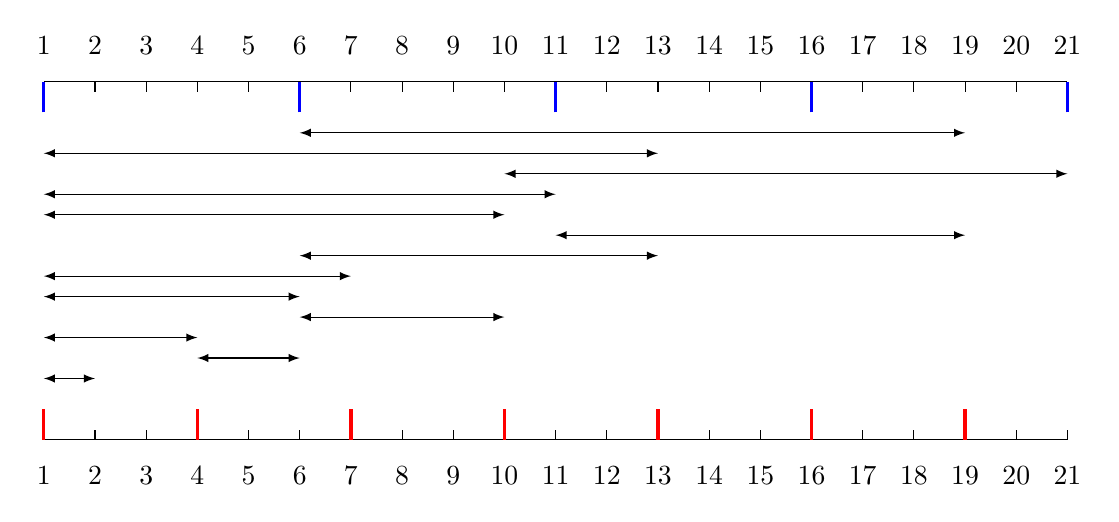
\begin{tikzpicture}[scale=1.3]

\draw (1,0) -- (11,0);

\draw [red, very thick] (1,0) -- (1,0.3);
\draw (1.5,0) -- (1.5,0.1);
\draw (2,0) -- (2,0.1);
\draw [red, very thick] (2.5,0) -- (2.5,0.3);
\draw (3,0) -- (3,0.1);
\draw (3.5,0) -- (3.5,0.1);
\draw [red, very thick] (4,0) -- (4,0.3);
\draw  (4.5,0) -- (4.5,0.1);
\draw (5,0) -- (5,0.1);
\draw [red, very thick] (5.5,0) -- (5.5,0.3);
\draw (6,0) -- (6,0.1);
\draw (6.5,0) -- (6.5,0.1);
\draw [red, very thick] (7,0) -- (7,0.3);
\draw (7.5,0) -- (7.5,0.1);
\draw (8,0) -- (8,0.1);
\draw [red, very thick] (8.5,0) -- (8.5,0.3);
\draw (9,0) -- (9,0.1);
\draw (9.5,0) -- (9.5,0.1);
\draw [red, very thick] (10,0) -- (10,0.3);
\draw (10.5,0) -- (10.5,0.1);
\draw (11,0) -- (11,0.1);

\node at (1,-0.35) {1};
\node at (1.5,-0.35) {2};
\node at (2,-0.35) {3};
\node at (2.5,-0.35) {4};
\node at (3,-0.35) {5};
\node at (3.5,-0.35) {6};
\node at (4,-0.35) {7};
\node at (4.5,-0.35) {8};
\node at (5,-0.35) {9};
\node at (5.5,-0.35) {10};
\node at (6,-0.35) {11};
\node at (6.5,-0.35) {12};
\node at (7,-0.35) {13};
\node at (7.5,-0.35) {14};
\node at (8,-0.35) {15};
\node at (8.5,-0.35) {16};
\node at (9,-0.35) {17};
\node at (9.5,-0.35) {18};
\node at (10,-0.35) {19};
\node at (10.5,-0.35) {20};
\node at (11,-0.35) {21};

\draw (1,3.5) -- (11,3.5);

\draw [blue, very thick] (1,3.2) -- (1,3.5);
\draw (1.5,3.4) -- (1.5,3.5);
\draw (2,3.4) -- (2,3.5);
\draw (2.5,3.4) -- (2.5,3.5);
\draw (3,3.4) -- (3,3.5);
\draw [blue, very thick] (3.5,3.2) -- (3.5,3.5);
\draw (4,3.4) -- (4,3.5);
\draw  (4.5,3.4) -- (4.5,3.5);
\draw (5,3.4) -- (5,3.5);
\draw (5.5,3.4) -- (5.5,3.5);
\draw [blue, very thick] (6,3.2) -- (6,3.5);
\draw (6.5,3.4) -- (6.5,3.5);
\draw (7,3.4) -- (7,3.5);
\draw (7.5,3.4) -- (7.5,3.5);
\draw (8,3.4) -- (8,3.5);
\draw [blue, very thick] (8.5,3.2) -- (8.5,3.5);
\draw (9,3.4) -- (9,3.5);
\draw (9.5,3.4) -- (9.5,3.5);
\draw (10,3.4) -- (10,3.5);
\draw (10.5,3.4) -- (10.5,3.5);
\draw [blue, very thick] (11,3.2) -- (11,3.5);

\node at (1,3.85) {1};
\node at (1.5,3.85) {2};
\node at (2,3.85) {3};
\node at (2.5,3.85) {4};
\node at (3,3.85) {5};
\node at (3.5,3.85) {6};
\node at (4,3.85) {7};
\node at (4.5,3.85) {8};
\node at (5,3.85) {9};
\node at (5.5,3.85) {10};
\node at (6,3.85) {11};
\node at (6.5,3.85) {12};
\node at (7,3.85) {13};
\node at (7.5,3.85) {14};
\node at (8,3.85) {15};
\node at (8.5,3.85) {16};
\node at (9,3.85) {17};
\node at (9.5,3.85) {18};
\node at (10,3.85) {19};
\node at (10.5,3.85) {20};
\node at (11,3.85) {21};

\draw [>=latex,<->] (1,0.6) -- (1.5,0.6);
\draw [>=latex,<->](2.5,0.8) -- (3.5,0.8);
\draw [>=latex,<->](1,1) -- (2.5,1);
\draw [>=latex,<->](3.5,1.2) -- (5.5,1.2);
\draw [>=latex,<->](1,1.4) -- (3.5,1.4);
\draw [>=latex,<->](1,1.6) -- (4,1.6);
\draw [>=latex,<->](3.5,1.8) -- (7,1.8);
\draw [>=latex,<->](6,2) -- (10,2);
\draw [>=latex,<->](1,2.2) -- (5.5,2.2);
\draw [>=latex,<->](1,2.4) -- (6,2.4);
\draw [>=latex,<->](5.5,2.6) -- (11,2.6);
\draw [>=latex,<->](1,2.8) -- (7,2.8);
\draw [>=latex,<->](3.5,3) -- (10,3);

\end{tikzpicture}
\caption{coprime sampling solution with $m=3$ and $n=5$}\label{tkz:coprime_ruler}
\end{figure}

\subsection{ci aanmaken}\label{sub:ci-coprime}
blaatverhaal
\end{document}
